\documentclass[]{beamer}

\usetheme{Ilmenau} %theme
\usecolortheme{beaver}

%Unipd Colors
\definecolor{unipd}{RGB}{155,0,20}

\setbeamercolor{structure}{fg=unipd}
\setbeamercolor{title}{fg=unipd}
\setbeamercolor{titlelike}{fg=unipd}

\usepackage[utf8]{inputenc} %utf-8 input
\usepackage{float}


\title{PastBot: un bot per la piattaforma Facebook Messenger per l'interazione con gli utenti}
\author[Davide Polonio]{
\includegraphics[width=0.6\textwidth]{logo.png}}
\date{13-10-2016}
\institute[Universit\`a degli studi di Padova]
          {
              Dipartimento di Matematica\\
              Corso di Laurea in Informatica\\
              Universit\`a degli studi di Padova
          }
          
\subject{Computer Science}

%\graphicspath{{res/img/}}

\addtobeamertemplate{navigation symbols}{}{%
    \usebeamerfont{footline}%
    \usebeamercolor[fg]{footline}%
    \hspace{1em}%
    \insertframenumber/\inserttotalframenumber
}

\setbeamercolor{footline}{fg=unipd}
\setbeamerfont{footline}{series=\bfseries}

\begin{document}
\graphicspath{ {res/img/} }

%\begin{frame}
%  \tableofcontents
%\end{frame}

%usage: \input{res/slide/whatDoYouWant}
%\input{res/slide/example}
\begin{frame}
  \titlepage
\end{frame}



%this is a example of a slide, don't include it in the project

\section{Introduzione}
\begin{frame}

  \frametitle{PastBot}

  \begin{figure}[H]
    \centering
    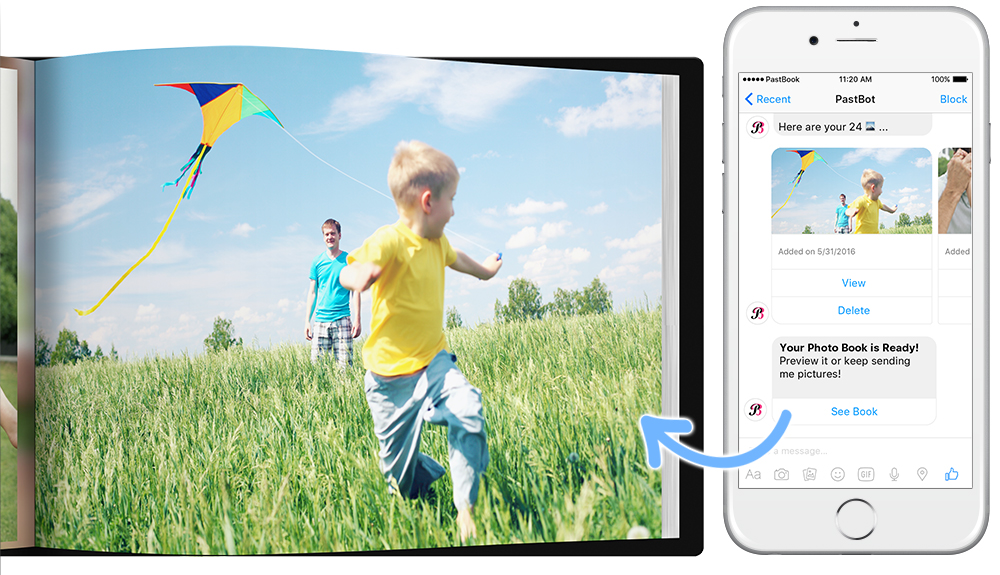
\includegraphics[scale=0.3]{PastBotLandingPage}
  \end{figure}

  %Qui posso parlare di che cos'e' e a cosa serve
  
\end{frame}

%this is a example of a slide, don't include it in the project

\section{Tecnologie}
\begin{frame}

  \frametitle{Tecnologie utilizzate}

  \begin{columns}
    \begin{column}{0.5\textwidth}
      
      \begin{itemize}
      \item Amazon AWS
        \begin{itemize}
        \item Lambda
        \item DynamoDB
        \item APIGateway
        \end{itemize}
      \item NPM
      \item Swagger
      \item Apex
      \item Messenger
      \item Dashbot
      \item Git
      \end{itemize}
    \end{column}
    \begin{column}{0.5\textwidth}
      \begin{figure}
        \centering
        
\includegraphics[scale=0.22]{Tec}
      \end{figure}
    \end{column}
  \end{columns}

  %content
  
\end{frame}

%this is a example of a slide, don't include it in the project

\section{Analisi dei requisiti}
\begin{frame}

  \frametitle{Analisi dei requisiti}

  \begin{itemize}
  \item Gestione album fotografici
  \item Gestione fotografie
  \item Richiesta di informazioni
  \item Ordinazione album
  \end{itemize}
  
\end{frame}

%this is a example of a slide, don't include it in the project

\section{Progettazione}
\begin{frame}

  \frametitle{Progettazione}

  %content
  
\end{frame}

%this is a example of a slide, don't include it in the project

\section{Codifica}
\begin{frame}

  \frametitle{Codifica e Test}

  \begin{itemize}
  \item Regole di scrittura
  \item Test effettuati tramite
    \begin{itemize}
    \item Mocha
    \item APIGateway
    \end{itemize}
  \end{itemize}

  \begin{figure}[H]
    \centering
    
\includegraphics[scale=0.45]{MochaLogo}
  \end{figure}

  %content
  
\end{frame}

%this is a example of a slide, don't include it in the project

\section{Codifica}
\begin{frame}

  \frametitle{Codifica e Test}

  \begin{itemize}
  \item Regole di scrittura
  \item Test effettuati tramite
    \begin{itemize}
    \item Mocha
    \item APIGateway
    \end{itemize}
  \end{itemize}

  \begin{figure}[H]
    \centering
    
\includegraphics[scale=0.45]{MochaLogo}
  \end{figure}

  %content
  
\end{frame}

%this is a example of a slide, don't include it in the project

\section{Titolo}
\begin{frame}

  \frametitle{Title}

  %content
  
\end{frame}



\end{document}
